\chapter{Hiện thực mô hình}

\section{Công cụ}

Trong quá trình hiện thực, nhóm cũng sử dụng các công cụ có sẵn để giúp ít cho việc huấn luyện mô hình, tăng hiệu suất lập trình. Nhóm sử dụng chủ yếu hai framework là Keras và Pytorch. Với nhiệm vụ phát hiện, bao đóng vật thể và segmentation, thì nhóm đã sử dụng mô hình có sẵn được viết bằng Keras của tác giả khác để sử dụng . Framework thứ hai mà nhóm sử dụng là Pytorch, ưu điểm của nó là có thể chạy linh động (dynamic), được nhóm dùng để hiện thực Fully Convolution Residuals Networks, cũng như kết hợp cả 2 mô hình trên nhằm mục tiêu dự đoán khoảng cách vật thể.

\subsection{Pytorch}
% mi viết cái ni nghe vũ
Pytorch là một framework được phát triển bởi Facebook. Pytorch sử dụng dynamic graph, đây là một tính năng khá có sức hút đối với các nhà nghiên cứu và kĩ sư thường làm việc với dữ liệu về time-series và xử lý ngôn ngữ tự nhiên. Pytorch được tạo ra để vận dụng các thư viện trên Torch, đưa các thư viện này lên ngôn ngữ Python để sử dụng giúp mở rộng sự phổ biến, vì Torch được sử dụng trên ngôn ngữ Lua nên ít được phổ biến. Pytorch được tích hợp với Python khá sâu và nó theo dạng hướng đối tượng. Pytorch cũng cho phép mở rộng các chức năng một cách dễ dàng bằng cách khai báo những lớp kế thừa Pytorch. Giả sử, khi muốn tạo ra một lớp neural network bằng cách chỉnh sửa từ một lớp neural network có sẵn thì có thể kế
thừa từ nn.Module. Pytorch cung cấp 3 mức ở dạng trừ tượng để giúp mọi thứ dễ dàng sử dụng. Tensor trong Pytorch bắt buộc ở dạng nd-array, nó cũng giống với numpy nhưng lại có thể chạy được trên GPU. Biến (variable) là node trong sơ đồ tính toán computational graph) nó rất giống với tensor, variable, placeholder trong Tensorflow. Module là neural network layer, có thể lưu trữ các trọng số (weights). Pytorch ra đời muộn nhưng lại rất phổ biến trong cộng đồng nghiên cứu.
\subsection{Keras}
Keras là framework về học sâu,là dạng API, được viết bằng Python, và có thể chạy với các backend: Tensorflow, Theano, CNTK. Keras là một framework dễ tiếp cận, sử dụng, cho phép người dùng lập trình một cách nhanh chóng, dễ đọc, không rườm rà. Đặc biệt, ta có thể dễ dàng mở rộng, thêm các components mới vào mô hình đã có. Mặt khác, Keras cũng hỗ trợ đầy đủ các lớp trong mạng CNN và mạng RNN, có thể chạy được trên đồng thời CPU, GPU.
\begin{comment}
\section{Công việc cần chuẩn bị cho quá trình huấn luyện mô hình}

\subsection{Xử lý dữ liệu}

Sau khi tìm hiểu các tập dữ liệu về ảnh RGB-D, nhóm quyết định chọn bộ dữ liệu NYUV2. Đây là bộ dữ liệu được thu thập bằng máy Microsoff Kinect, với rất nhiều ngữ cảnh trong nhà khác nhau. Tập dữ liệu gồm 2 phần chính, đó là tập dữ liệu thô lên đến 407204 ảnh, và tập dữ liệu đã được đánh nhãn với 1449 ảnh. Với mục tiêu chính nhằm mục đích hiểu, có thể phân tích và đánh giá các mô hình dự đoán ảnh độ sâu, đồng thời với những khó khăn về phần cứng, nhóm quyết định chủ yếu sẽ tiến hành thí nghiệm trên tập dữ liệu nhỏ đã đánh nhãn với 1449 ảnh. 

\section{Quá trình huấn luyện mạng FCRN}
\subsection{Tài nguyên sử dụng}
Để tăng tốc quá trình huấn luyện nhóm đã sử dụng một GPU NVIDIA GTX 1080 có dung lượng ram là 8GB. Việc dùng GPU thay cho CPU nhằm tận dụng được khả năng tính toán song song vượt trội mà GPU mang lại.
\subsection{Kế hoạch huấn luyện}
\end{comment}
\section{Hiện thực mô hình ước lượng độ sâu và tiến hành thí nghiệm}
\subsection{Xử lý dữ liệu}

%Sau khi tìm hiểu các tập dữ liệu về ảnh RGB-D, nhóm quyết định chọn bộ dữ liệu NYUV2 \cite{silberman2012indoor}. Đây là bộ dữ liệu được thu thập bằng máy Microsoff Kinect, với rất nhiều ngữ cảnh trong nhà khác nhau. Tập dữ liệu gồm 2 phần chính, đó là tập dữ liệu thô lên đến 407204 ảnh, và tập dữ liệu đã được đánh nhãn với 1449 ảnh. Với mục tiêu chính nhằm mục đích hiểu, có thể phân tích và đánh giá các mô hình dự đoán ảnh độ sâu, đồng thời với những khó khăn về phần cứng, nhóm quyết định chủ yếu sẽ tiến hành thí nghiệm trên tập dữ liệu nhỏ đã đánh nhãn với 1449 ảnh. 
Sau khi tìm hiểu các tập dữ liệu về ảnh RGB-D, nhóm quyết định chọn bộ dữ liệu NYU-Depth V2 \cite{silberman2012indoor}. Đây là bộ dữ liệu được thu thập bằng máy Microsoff Kinect, với rất nhiều khung cảnh trong nhà khác nhau. Nó có đặc điểm:
\begin{itemize}
\item Tập dữ liệu được đánh nhãn có 1449 cặp ảnh gồm ảnh RGB và ảnh độ sâu tương ứng.
\item Có 464 khung cảnh khác nhau
\item Tập dữ liệu thô có số lượng ảnh lên đến 407204 ảnh.
\end{itemize}
Với mục tiêu chính nhằm mục đích hiểu, có thể phân tích và đánh giá các mô hình dự đoán ảnh độ sâu, đồng thời với những khó khăn về phần cứng, nhóm quyết định chủ yếu sẽ tiến hành thí nghiệm trên tập dữ liệu đánh nhãn.
\subsubsection{Tập dữ liệu đánh nhãn}
Tập dữ liệu này là tập con của tập dữ liệu thô. Nó bao gồm các cặp ảnh RGB và ảnh độ sâu cùng với một tập nhãn dày tương ứng, thêm vào đó ảnh độ sâu này đã được tiền xử lí để những giá trị độ sâu bị thiếu được điền đầy đủ bằng cách sử dụng  colorization scheme of Levin et al. \cite{nyu}
\begin{center}
         \begin{figure}[H]
         \begin{center}
           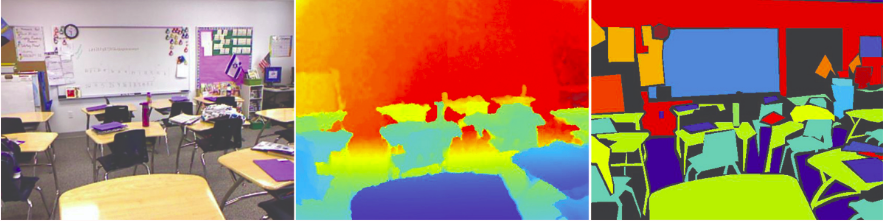
\includegraphics[scale=0.5]{image/nyu}
          \end{center}
          \caption{ảnh RGB (trái), ảnh độ sâu đã được xử lí (giữa), một tập các nhãn (phải) cho bức ảnh }
          \label{ref_sigmoid}
          \end{figure}
 \end{center}
 
 Tập dữ liệu này đã được chia làm 2 phần, gồm có 795 ảnh cho quá trình huấn luyện và 654 ảnh cho quá trình kiểm tra, nhận thấy tập kiểm tra chiếm 45\% của toàn bộ tập dữ liệu, nên nhóm tiến hành chia lại tập dữ liệu sao cho quá trình huấn luyện chiếm khoảng 80\% tập dữ liệu, thành 3 phần bằng cách lấy ngẫu nhiên 205 ảnh của tập kiểm tra bổ sung và tập huấn luyện và lấy thêm 159 ảnh cũng từ tập kiểm tra để tạo một tập xác thưc (validation set). Cuối cùng nhóm có tập huấn luyện có 1000 ảnh, tập xác thực có 159 ảnh và tập kiểm tra có 290 ảnh. Các ảnh này ban đầu có kích thước là 640$\times$480 sau đó được giảm xuống còn một nửa và tiến hành lấy trung tâm (center crop) để cuối cùng có kích thước là 304$\times$228.
\subsection{Thí nghiệm}
Mô hình deep regression network được hiên thực trên PyTorch,
\subsubsection{Tài nguyên sử dụng}
Nhóm đã sử dụng một GPU NVIDIA GTX 1080 có dung lượng RAM là 8GB nhằm tận dụng khả năng tính toán song song mà GPU hỗ trợ để tăng tốc quá trình huấn luyện.
\subsubsection{Chiến lược huấn luyện}
Trong quá trình huấn luyện nếu chỉ sử dụng ảnh RGB làm đầu vào thì phần trọng số của ResNet ở những lớp encoding sẽ được khởi tạo bằng trọng số ResNet đã được huấn luyện trên tập dữ liệu ImageNet \cite{Imagenet}. Còn đối với việc huấn luyện sử dụng đầu vào là ảnh RGB và ảnh độ sâu thưa thì đầu vào sẽ có 4 chiều RGB-D, nên lớp đầu tiên sẽ có channel vào (inchannels) là 4 do đó trọng số sẽ được khởi tạo theo phân phối Gaussian như sau:
\begin{itemize}
\item Nếu lớp cần được khởi tạo là một lớp convolution thì  $ w \sim  N( \mu = 0,\sigma ^{2} = \frac{2}{n} )$ với $n$ là tích của chiều dài, chiều rộng của kernel và số kernel của lớp đó.
\item Nếu lớp cần được khởi tạo là một lớp deconvolution thì $ w \sim  N( \mu = 0,\sigma ^{2} = \frac{2}{n} )$ $n$ là tích của chiều dài, chiều rộng của kernel và số channel của feature map của lớp trước của lớp đó.
\end{itemize}

Cách trên còn được áp dụng để khởi tạo các lớp deconvolution hoặc các lớp convolution của khối Up-projection thuộc các lớp decoding của mạng. Sau đây là các  siêu tham số (hyperparameter) mà nhóm đã thực hiện trong qúa trình huấn luyện. Số lượng mỗi bó (batchsize) trong quá trình huấn luyện là 8, tối ưu bằng phương pháp SGD với momentum\cite{momentum} với hệ số momentum là 0.9, hệ số học (leaning rate) ban đầu là 0.01 cứ sau 10 epoch sẽ giảm 10 lần. Hệ số weight decay là $10^{-4}$ được áp dụng để chính quy hóa (regularization).
Trong quá trình huấn luyện nhóm sẽ tiến hành đánh giá chất lượng mô hình sau mỗi epoch trên tập xác thực (valadation set) thông qua các độ đo được trình bày ở chương 6. Kết thúc quá trình huấn luyện thì mô hình cho kết quả tốt nhất trên tập xác thực sẽ được giữ lại.


\section{Quá trình ước lượng khoảng cách của vật thể}

Sau khi có được mô hình FCRN, nhóm sẽ tiến hành kết hợp kết quả của mô hình này với Mask RCNN nhằm ước lượng khoảng cách vật thể. Theo như nhóm đã trình bày trong hướng tiếp cận, việc ước lượng sẽ được thực hiện theo 4 phương án:
% một là dựa trên kết quả phát hiện bao đóng vật thể, tiến hành lấy các điểm mẫu bằng các phân bố ngẫu nhiên những điểm xung quanh tâm bao đóng của vật thể và kết quả depth map từ FCRN để ước lượng. Hướng thứ hai là sử dụng kết quả segmentation, lấy toàn bộ những pixel thuộc vật thể và kết quả depth map từ FCRN để ước lượng.
\subsection{Ước lượng khoảng cách bằng các điểm nằm trong bao đóng của vật thể}
Theo hướng này, chúng ta sẽ lấy tất cả những điểm nằm trong bao đóng của vật thể để ước lượng khoảng cách. Ví dụ: kết quả bao đóng từ Mask RCNN: [(x1,y1), (x2,y2)] = [(228,223), (255,283)], vậy, nhóm sẽ lấy tất cả những điểm có tọa độ thỏa mãn: $x \in (228,255)$  $\&$ $y \in (223,283).$ Dựa trên tọa độ của những điểm được chọn và ảnh độ sâu, ta sẽ có ước lượng khoảng cách của tất cả những điểm nằm trong bao đóng vật thể. Từ đây, nhóm quyết định lấy trung bình tất cả các giá trị khoảng cách này khoảng cách từ camera đến vật thể. Ngoài ra, các giá trị lớn nhất, nhỏ nhất của các giá trị độ sâu này cũng được ghi lại, nhằm đánh giá sự ảnh hưởng các các điểm nằm trong bao đóng nhưng không thuộc vật thể. 

\subsection{Ước lượng khoảng cách bằng lấy mẫu những điểm  xung quanh tâm bao đóng của vật thể, theo phân bố Gaussian.}

Đầu tiên, nhóm sẽ tiến hành khởi tạo ngẫu nhiên  1000 điểm theo phân bố Gaussian $ X_{random} \sim  N( \mu = (0,0),\sigma ^{2} = 1 )$ theo cả trục x, y. Tiếp theo, dựa vào kết quả bao đóng vật thể của Mask RCNN, lấy điểm chính giữa bao đóng làm $\mu$ của phân bố, chuyển đổi 1000 điểm đã khởi tạo được theo tỉ lệ của bao đóng. Ví dụ: Kết quả bao đóng từ Mask RCNN: (x1,y1) = (83,147);(x2,y2) = (264,419). Ta sẽ tìm được tâm bao đóng N($x_{center}$ = 173.5,$y_{center}$ = 283), kích thước bao đóng: chiều dài = y2-y1 = 117, chiều rộng =  264 - 83 = 181. Bên cạnh đó, theo tính chất của phân bố Gaussian, thì tọa độ của  những điểm phân bố $X_{random} \in (-3\sigma, 3\sigma)$, dựa vào tỉ lệ giữa kích thước bao đóng và giới hạn tọa độ của những điểm thuộc phân bố Gaussian, đưa tọa độ những điểm $X_{random}$ về tỉ lệ kích thước của bao đóng. Tọa độ mới của những điểm này được làm tròn lên. Hình \ref{fig:gaussian_to_bbbox} là kết quả của việc chuyển đổi từ những điểm random của phân bố Gaussion theo kích thước bao đóng của vật thể. 

\begin{figure}[H]%
    \centering
    \subfloat[Gaussian Distribution]{{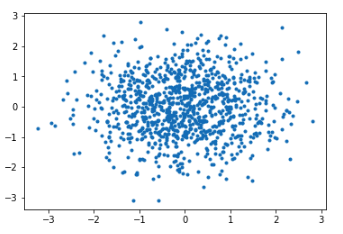
\includegraphics[height=5cm,width=7cm]{image/gaussdistribution} }}%
    \qquad
    \subfloat[Gaussian Distribution to bouding box]{{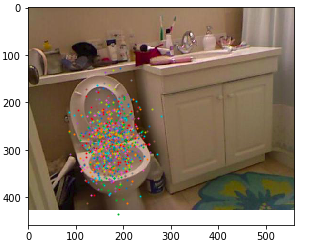
\includegraphics[height=5cm,width=7cm]{image/map_gaudis} }}%
    \caption{ \small a) Kết quả khởi tạo ngẫu nhiên  điểm theo phân bố Gaussian $ X_{random} \sim  N( \mu = (0,0),\sigma ^{2} = 1 )$.\\ b) Kết quả chuyển đổi tọa độ các điểm phân bố đến bao đóng vật thể 
    }
    \label{fig:gaussian_to_bbbox}%
\end{figure}

 
\subsection{Ước lượng khoảng cách dựa trên kết quả phân đoạn của Mask RCNN}
Dựa vào kết quả phân đoạn của Mask RCNN, ta sẽ có những điểm mà Mask RCNN cho là thuộc về vật thể. Kết hợp những điểm này với kết quả ảnh độ sâu từ FCRN, ta sẽ có giá trị độ sâu của tất cả những điểm thuộc về vật thể. Từ đây, lấy giá trị trung bình của tất cả những điểm trên làm giá trị khoảng cách vật thể.


\subsection{Ước lượng khoảng cách bằng cách lấy mẫu những điểm xung quanh tâm bao đóng của vật thể theo phân phối Gaussian, trong đó những điểm này phải được Mask RCNN cho là thuộc về vật thể}
Từ phương án 2, nhóm đã có danh sách những điểm thuộc về bao đóng vật thể, những điểm mà được chuyển đổi từ phân bố Gaussian. Trong những điểm này, nhóm chỉ lấy những điểm mà Mask RCNN cho là thuộc về vật thể. Sau khi có tập những điểm cuối cùng, lấy giá trị độ sâu của những điểm này từ ảnh độ sâu, và tiến hành tính giá trị khoảng cách bằng giá trị trung bình. 



% Qua quá trình tìm hiểu về các mô hình nhận diện vật thể, nhóm quyết định tìm hiểu sâu hơn về mô hình Faster R-CNN. Hiện tại, nhóm tham khảo và đang tiến hành nghiên cứu và chạy Faster R-CNN với mô hình VGG16 trên tập dữ liệu NYUV2 để tiến hành phát hiện vật thể. \\

% Với tập dữ liệu PASCALVOC2007 và mô hình VGG16 đã được huấn luyện sẵn, kết quả của bao đóng vật thể cho kết quả rất tốt.

% \begin{figure}[H]%
%     \centering
%     \subfloat[Detect person]{{\includegraphics[height=5cm,width=7cm]{image/example1} }}%
%     \qquad
%     \subfloat[Detect dog]{{\includegraphics[height=5cm,width=7cm]{image/example2} }}%
%     \caption{A cartoon drawing of a biological neuron (left) and its mathematical model (right).}%
%     \label{fig:example}%
% \end{figure}


% %chỗ này ta đang tiến hành train, trước mắt chưa có kết quả lập tức được. sẽ dán hình chỗ này sau.

% \section{Tiềm năng}

% Việc xác định vật thể trong không gian 3 chiều sẽ được ứng dụng vào trong nhiều lĩnh vực cũng như hệ thống, trong đó nổi bật nhất chính là phục vụ cho robot.
% \begin{itemize}
% \item Giúp robot có thể hiểu được kích cỡ vật thể, có thể tiến hành thao tác chính xác hơn.
% \item Với xe tự lái, khi có thể hiểu được ngữ cảnh 3 chiều, nó có thể biết được khoảng cách giữa các đối tượng để có thể tiến hành điều chỉnh hợp lí, phù hợp với tình trạng giao thông hiện tại.

% \end{itemize}

% \section{Khó khăn}

% Hiện tại, việc phát hiện vật thể trong không gian 2 chiều đã được nhóm tìm hiểu và đang tiến hành huấn luyện. Nhưng với mục tiêu có thể bao đóng vật thể trong không gian 3 chiều, nhóm vẫn còn gặp nhiều khó khăn.

% \begin{itemize}
% 	\item Nhóm có tìm hiểu các dataset về ảnh RGB-D như: SUN RGBD, NYUV2... và thấy NYUV2 khá tốt, đặc biệt đã có hiệu chỉnh về ảnh độ sâu. Về việc tự thu thập dữ liệu, ở đây là ảnh RGB-D bằng máy Kinect, nhóm vẫn chưa tìm hiểu cũng như tiến hành chụp ảnh. Ngoài ra, ảnh độ sâu thu được cũng thường bị nhiễu và cần phải điều chỉnh, tăng chất lượng của ảnh. 
%     \item Các bài báo nói về việc thực hiện bao đóng vật thể trong không gian 3 chiều khá khó hiểu, đồng thời đòi hỏi nhiều kiến thức khá phức tạp. Do vậy, nhóm còn khá mập mờ về phần này. Trong giai đoạn luận văn, nhóm sẽ cố gắng tìm hiểu kĩ hơn cũng như tham khảo ý kiến của thầy hướng dẫn để có thể hoàn thành mục tiêu của đề tài.
%     \item Về tài nguyên cho việc huấn luyện để thực hiện phát hiện vật thể trong không gian 2 chiều, hiện tại, nhóm đang tự huấn luyện bằng CPU để có thể dễ tiến hành điều chỉnh nên tốc độ huấn luyện khá chậm. Trong thời gian tới, nếu kết quả huấn luyện trên CPU khả quan hơn,  nhóm sẽ tiến hành huấn luyện trên tài nguyên mà thầy hướng dẫn cung cấp.
% \end{itemize}
% \section{Định hướng luận văn}
% Trong giai đoạn luận văn, nhóm sẽ tiến hành các công việc sau:
% \begin{itemize}
% \item Xác định rõ ràng hướng tiếp cận của nhóm.
% \item Thu thập dữ liệu từ máy Kinect, điều chỉnh dữ liệu, kết hợp với NYUV2 dataset.
% \item Hoàn thiện việc phát hiện vật thể trong không gian 2 chiều với dataset của nhóm.
% \item Tiến hành nghiên cứu nhiều hơn để có thể hiểu việc phát hiện vật thể trong không gian 3 chiều.
% \item Hiện thực mô hình để có thể phát hiện vật thể trong không gian 3 chiều.
% \end{itemize}
